\chapter{Conversational Search Assistant}
\label{chapter:CSA}


The {\ehden} portal provides a catalogue of medical databases across Europe, offering researchers a centralized platform to explore available medical data sources. {\ehden} built Network Dashboards tool to offer statistical and aggregated information about the databases available on the network. This tool helps researchers to choose the best databases across the catalogue. However, with the increasing number of databases in the catalogue, the process of find the most suitable databases becames difficult and time-consuming for a researcher.

This chapter focuses on the second goal of this dissertation: develop a chat-like search engine to help discover the best databases for a study. The following sections describes how the {\ehden} Catalogue search assistant and its components were implemented and the decisions and steps made over time.

% vamos falar sobre os dados, information retrieval, {\llm} e frameworks

\section{Data}
\label{data}
% sao os dados que usaste
% o artigo do cbms CAT
% tudo o que é relacionado com dados

The data utilized for this project comprises real {\ehden} data sourced from the catalogue and the Network Dashboards. There are four main files that contain the data necessary to obtain an overview of the databases available in the {\ehden} network: the countries file, the data sources file, the medical concepts file, and the Achilles Results file\footnote{\url{https://github.com/EHDEN/CatalogueExport}}. It is essential to understand the content of each file and the relationships between their data, as illustrated in Figure~\ref{fig_data_diagram}.

\begin{figure}[H]
    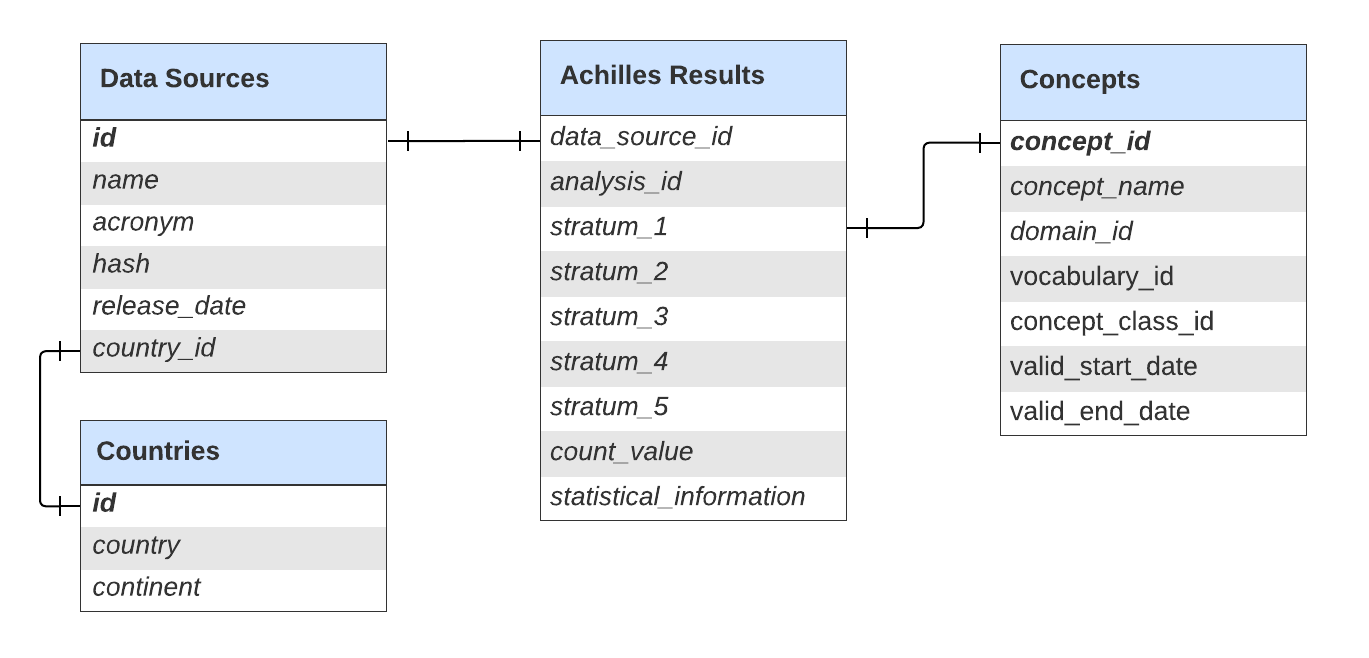
\includegraphics[width=1\textwidth]{figs/chapter3/data_diagram.png}
    \centering
    \caption[The diagram of the connection between the data files]{The diagram of the connection between the data files.}
    \label{fig_data_diagram}
\end{figure}


To comprehend the purpose of the four files, each is detailed with fields, description and an example of entries~\cite{almeida2024healthdbfinder}. When the data is private and sensitive, not-real examples are included to better understand the content and connections between files.

\paragraph{Countries file {\small\normalfont(\texttt{countries.csv})}}

\begin{itemize}
    \item \textbf{Fields:} \texttt{id}, \texttt{country}, \texttt{continent}.
    \item \textbf{Description:} This file contains of real-world data, listing countries and their corresponding continents. It is used to provide geographical context for the analyzes, and supporting studies that require demographic segmentation.
    \item \textbf{Example Entries:}
    \begin{itemize}
        \item \texttt{233, Ukraine, Europe}
        \item \texttt{149, Montenegro, Europe}
    \end{itemize}
\end{itemize}


\paragraph{Data sources file {\small\normalfont(\texttt{data\_sources.csv})}}

\begin{itemize}
    \item {\raggedright\textbf{Fields:} \texttt{id}, \texttt{name}, \texttt{acronym}, \texttt{hash}, \texttt{release\_date}, \texttt{country\_id}.\par}
    \item \textbf{Description:} This file includes essential details of the databases such as the source identification, the database name and the hash code of the {\ehden} catalogue.
    \item \textbf{Example Entries:}
    \begin{itemize}
        \item \texttt{1, MEDIBASE, Medical Database for Health Information Exchange, <hash>, NA,107}
        \item \texttt{2, GRAVITAS, Global Repository of Advanced Vaccine Innovations Technologies and Strategies, <hash>, NA, 228}
    \end{itemize}
\end{itemize}

\paragraph{Medical concepts file {\small\normalfont(\texttt{concepts.csv})}}

\begin{itemize}
    \item {\raggedright\textbf{Relevant fields:}
    \texttt{concept\_id}, \texttt{concept\_name}, \texttt{domain\_id}, \texttt{vocabulary\_id}.\par}
    \item \textbf{Description:} The concepts file contains metadata on medical concepts, extracted from OHDSI Athena\footnote{\url{https://athena.ohdsi.org/}}.
    \item \textbf{Example Entries:}
    \begin{itemize}
        \item \texttt{2966436, Latanoprost (Apotex) 0.005\% Eye Drops 2.5 Ml Bottle, Drug, AMT, Containered Pack, NA, 1009551000168106, 2016-11-01, 2099-12-31, NA}
        \item \texttt{2966944, Letrozole (Apotex) 2.5 Mg Tablet, Drug, AMT, Trade Product Unit, NA, 1009571000168102, 2016-11-01, 2099-12-31, NA}
    \end{itemize}
\end{itemize}

\paragraph{Database summaries {\small\normalfont(\texttt{achilles\_results.csv})}}

\begin{itemize}
    \item {\raggedright\textbf{Relevant fields:} \texttt{data\_source\_id}, \texttt{analysis\_id}, \texttt{stratum\_n (from 1 to 5)}, \texttt{count\_value}, \texttt{statistical information}.\par}
    \item \textbf{Description:} Metadata summary of metadata present in the databases providing aggregated analytics. The “stratum\_1” field points to the concept ID. 
    \item \textbf{Example Entries:}
    \begin{itemize}
        \item \texttt{143, 1, NA, 8507.0, NA, NA, NA,988296, NA, NA, NA, NA, NA, NA, NA, NA, NA}
        \item \texttt{138, 2, 8532.0, 8532.0, NA, NA, NA, 1354216, 526.0, 52600.0, 26300.0, 52.6, 25774.0, 52.6, 157.79, 368.2, 499.7}
    \end{itemize}
\end{itemize}

\hspace{1cm}

The combination of these four files gives the necessary information about the databases. Each row of the Achilles Results file contains statistical information about each concept available in the database, and a set of characteristics that are commonly used to filter databases in a cohort study. For instance, the number of samples segregated by range of age. 


\section{Information Retrieval}

\hl{To to gain more knowledge about implementing {\ir} methods and, at the same time, validate the {\ir} results of this dissertation, I was involved in a challenge, BioASQ\footnote{\url{http://bioasq.org/}}. BioASQ addresses the information access problem for biomedical experts by organizing challenges in biomedical semantic indexing and {\qa}. These challenges cover tasks such as hierarchical text classification, machine learning, {\ir}, {\qa} from texts and structured data, and multi-document summarization.}

This section outlines the {\ir} component, covering the BioASQ challenge and its relevance, and the implementation of BM25 for indexing and searching databases.


\subsection{BioASQ challenge 2024}
\label{bioasq}

The BioASQ includes several challenges. My team was involved in ``BioASQ Task 12b'', focusing on biomedical semantic {\qa}. This challenge aims to advance the development of systems capable of understanding and answering biomedical questions. Participants must respond to test questions using various types of information, including relevant concepts, articles, and snippets. The challenge involves 5,000 training questions with gold-standard answers and introduces 500 new test questions, all constructed by European biomedical experts. 

The challenge consists of two phases, A and B:

\begin{itemize}
    \item \textbf{Phase A}: Participants respond to released questions with relevant articles and snippets.
    \item \textbf{Phase B}: Participants provide exact and ideal answers based on questions and provide relevant articles and snippets.
\end{itemize}

My task was implementing and testing some {\ir} methods to determine which performs better. This task allowed me to have more concrete results. The techniques used and tested were {\bm}, SPLADE~\cite{formal_splade_2021}, and BGE-M3~\cite{chen_bge_2024}. As {\bm} has already been explained in the section~\ref{bm25}, here is a brief overview of the other methods tested.


\subsubsection{SPLADE} 

SPLADE\footnote{\url{https://github.com/naver/splade}} is a neural retrieval model that learns query/document sparse expansion through the {\bert} Masked Language Model head and sparse regularization, according to~\citet{formal_splade_2021} . This technique belongs to {\lsr} because it combines elements of traditional sparse retrieval techniques with machine learning, particularly deep learning. 

SPLADE is designed to balance the effectiveness of dense retrieval models with the interpretability and efficiency of sparse representations. It is advantageous  because it combines the benefits of dense and sparse models~\cite{formal_splade_2021}. This method can improve the relevance and accuracy of the search results, particularly in complex queries where understanding the context and the semantic relationships between terms is essential. The model used was \texttt{naver/splade-cocondenser-ensembledistil}, proposed by~\citet{formal_distillation_2022}.

% tbd


\subsubsection{BGE-M3} 

~\citet{chen_bge_2024} proposed the technique BGE-M3\footnote{\url{https://github.com/FlagOpen/FlagEmbedding/tree/master/FlagEmbedding/BGE_M3 }}. It is a versatile technique because it can perform three common retrieval functions: dense retrieval, multi-vector retrieval, and sparse retrieval. Also, this technique is multilingual because it supports over 100 languages and is multi-granular because it can process inputs ranging from short sentences to long documents, accommodating up to 8192 tokens. The model used was \texttt{BAAI/bge-m3} with 1024 of dimension and 8192 tokens of sequence length.


% tbd


\subsection{BM25 implementation}
\label{bm25implementation}

Although we have tested various methods, the implementation of {\bm} has shown promising results. {\bm} is the selected method for implementing the {\ir} component in this project. The library implemented was PyTerrier\footnote{\url{https://github.com/terrier-org/pyterrier}}, a Python framework for performing {\ir} experiments.


\subsubsection{Database indexing process}

The {\ir} component must index a collection of documents that thoroughly represent all the concepts within the databases, ensuring a clear understanding of what each database encompasses. To achive this, the data mentioned in the Section~\ref{data} is used to create the documents.

Figure~\ref{fig_struct} represents the different stages of the data. The first part of the figure, A), represents the three data files detailed in the Section~\ref{data}. These are received from the {\ehden} Network Dashboard. One contains information about the data sources, another contains the metadata summary of the databases (Achilles Results), and the last contains all medical concepts used in this community. These three files data was combined and readjusted to be indexed as documents. The remaining parts of this figure (B and C) represent the strategies adopted to create the documents of each database.

\begin{figure}[H]
    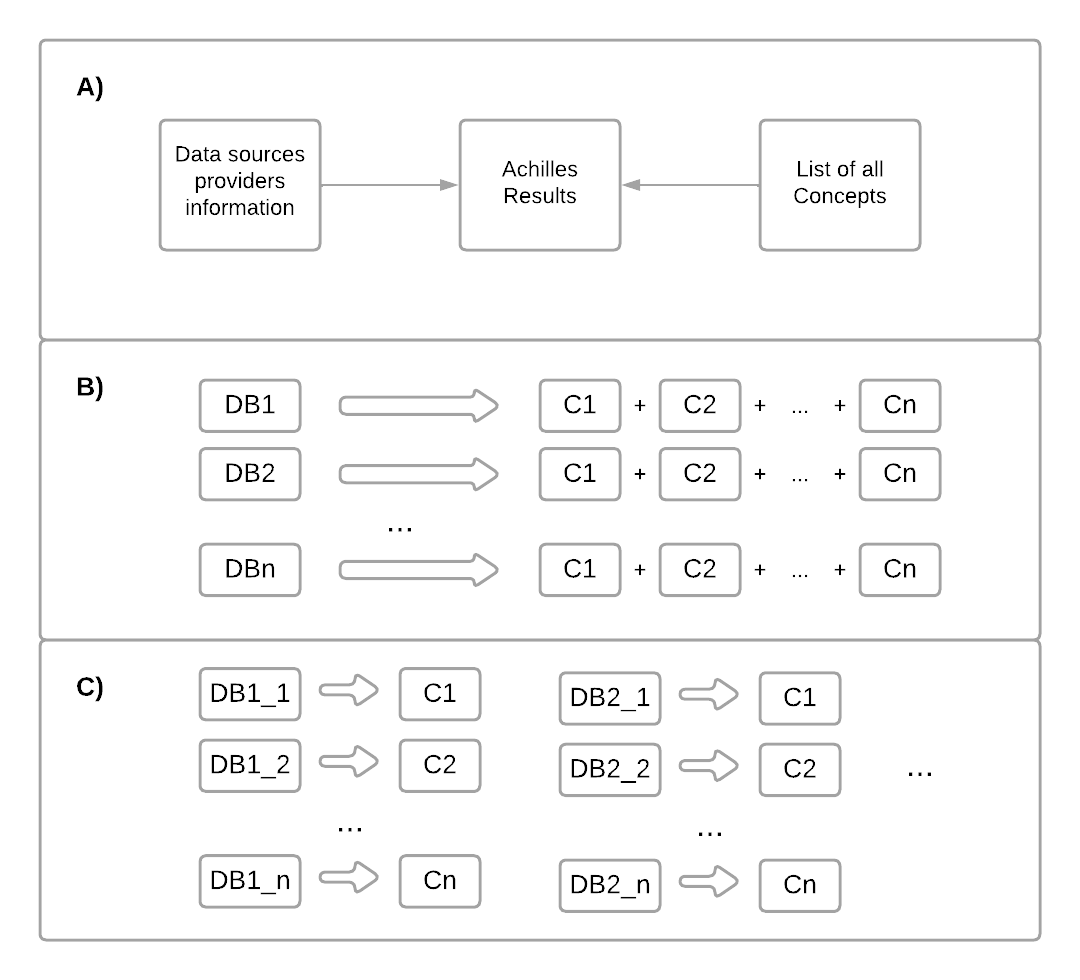
\includegraphics[width=0.8\textwidth]{figs/chapter3/index_struct.png}
    \centering
    \caption[Index data structure]{Index data structure: A) Metadata about the databases, B) First approach to the structure of indexed documents, C) Current approach to the structure of indexed documents.}
    \label{fig_struct}
\end{figure}


The first approach to structure of the documents to be indexed is shown in Figure~\ref{fig_struct}, part B). The document structure consists of a pairing of database IDs with their corresponding content. The content is represented as a single string, where each concept from each database is concatenated and separated by spaces. However, this way of indexing the database contents has several drawbacks: 

\begin{itemize}
    \item \textbf{Lack of Granularity}: By concatenating all concepts into a single string, the individual relevance of each concept is lost. When a search query is made, the search engine treats the entire string as a single document, reducing search results' precision and recall.
    \item \textbf{Poor Search Results}: The search engine returns unsatisfactory results because the indexing does not accurately reflect the importance of each concept. This leads to low search scores, resulting in commonly retrieving irrelevant documents.
\end{itemize}

The approach to creating the document structure has been refined to enhance the granularity and searchability of the database content. Each concept in the database is individually indexed, as shown in Figure~\ref{fig_struct}, part C). \hl{Each concept within a database is treated as a separate document for indexing purposes. This is achieved by assigning a document number that uniquely combines the database ID and the concept's position within its list. The document number serves as a unique identifier for each concept, ensuring that each piece of data can be individually retrieved and queried. The content of each document, represented by the concept itself, allows for reflecting the importance of concepts within the database, facilitating more precise and efficient retrieval of information.}


\subsubsection{Database searching process}
\label{searchprocess}

When the {\ir} system receives a query in free text, the system processes it using {\nlp} techniques applied to the query to enhance the search performance. These processes can include tokenization (splitting the text into individual terms or words), stemming or lemmatization (reducing words to their base form), and stop-word removal (eliminating common words that do not contribute to the search). \hl{Standarding the text and transforming the query into important terms improves the match between the queries and indexed concepts as documents.}

After processing the query, the {\bm} algorithm evaluates the relevance of each concept within the database to the query, assigning a score that reflects its relevance. The method returns the 100 most relevant results and scores each concept. Then, these concepts are grouped by databases. The total relevance score for each database is calculated by summing the scores of its concepts. This comprehensive compilation process highlights the most relevant concepts. To ensure that only the most pertinent databases are presented to the user, the engine applies a predefined threshold to filter out databases with lower cumulative scores. The remaining results are then sorted in descending order of their total scores, prioritizing those with the highest relevance to the query.

Each element in the ranked list of databases contains some information about the databases. The ranked databases have a unique numeric identifier, the respective database name, and the hash that identifies a database in the {\ehden} Catalogue. Also, it includes the total relevance score assigned to a database by the {\bm} algorithm, indicating how well the database matches the query. At last, the concepts that has been identified are also included.



\section{Large Language Model}
\label{sec:llm}

The {\llm} used in this project is \texttt{Nous Hermes 2 Mixtral 8x7B}~\cite{Nous-Hermes-2-Mixtral-8x7B-DPO} open model, finetuned from Mixtral~\cite{jiang2024a}. This model belongs to the llama family and has 47B of parameters. The reason for using this {\llm} model is that it is a promising model. The {\llm} is installed on a local version of the Ollama\footnote{\url{https://ollama.com/}} framework and deployed in a Virtual Machine to access the {\llm} using a URL. The model {\gpt} cannot be used for this project, due to the use of sensitive data. Since {\gpt} is not open-source, the data falls out of control.  It raises privacy concerns for private data in public services.


\subsection{Tasks}

The {\llm} has two types of tasks: text generation ({\nlg}) and text analysis ({\nlu}) . Table~\ref{table_tasks} shows the different tasks given to the LLM and the respective descriptions. Also, it presents the output format and the temperature used in each task. The output format is the generated response format expected from {\llm}. The temperature of a {\llm} refers to a hyperparameter that controls the randomness of predictions made by the model. A higher temperature results in more creative and random outputs. Otherwise, a lower temperature results in more deterministic and focused outputs.

\begin{table}[H]
  \centering
  \def\arraystretch{1.5}
  \resizebox{\textwidth}{!}{%
  \begin{tabular}{|c|c|l|}
  \hline
  \textbf{Type of Task}       & \textbf{Task}           & \textbf{Description}                                                                                                                                      \\ \hline
  \multirow{3}{*}{{\nlg}} & Generate response                & Generate a response to a given message.                                                                                                                   \\ \cline{2-3} 
                              & Generate response with databases & Generate a response to retrieve the best databases to the user.                                                                                           \\ \cline{2-3} 
                              & Generate question                & Generate a question related to a given question.                                                                                                          \\ \hline
  \multirow{3}{*}{{\nlu}}    & analyze topic                   & \begin{tabular}[c]{@{}l@{}}Identify if the user message is related to health. \\ If so, identify the research topic in the field of health.\end{tabular} \\ \cline{2-3} 
                              & analyze yes or no answer        & Indentify if the answer is positive or negative for a respective question.                                                                                \\ \cline{2-3} 
                              & analyze answer to question      & indentify if the answer is a response for a respective question.                                                                                          \\ \hline
  \end{tabular}%
  }
  \caption[Overview of the Large Language Model tasks]{Overview of the LLM tasks.}
  \label{table_tasks}
\end{table}


\subsection{LLM configuration and implementation}

After defining the tasks, Table~\ref{tasks_info} clarifies the parameters and the output format of each task.


\begin{table}[H]
  \centering
  \def\arraystretch{1.2}
  \resizebox{0.9\textwidth}{!}{%
  \begin{tabular}{|c|c|c|c|}
  \hline
  \textbf{Type of Task}       & \textbf{Task}           & \textbf{Output format}       & \textbf{\begin{tabular}[c]{@{}c@{}}Temperature\\ (0 - 1)\end{tabular}} \\ \hline
  \multirow{3}{*}{{\nlg}} & Generate response                & \multirow{3}{*}{Plain text}  & 0.4                                                                   \\ \cline{2-2} \cline{4-4} 
                              & Generate response with databases &                              & 0.4                                                                    \\ \cline{2-2} \cline{4-4} 
                              & Generate question                &                              & 0.4                                                                   \\ \hline
  \multirow{3}{*}{{\nlu}}    & analyze topic                   & \multirow{3}{*}{JSON object} & 0.1                                                                    \\ \cline{2-2} \cline{4-4} 
                              & analyze yes or no answer        &                              & 0.1                                                                    \\ \cline{2-2} \cline{4-4} 
                              & analyze answer to question      &                              & 0.1                                                                    \\ \hline
  \end{tabular}%
  }
  \caption[Large Language Model parameters and output information]{LLM parameters and output information.}
  \label{tasks_info}
\end{table}

Inside the generation main task, the {\llm} can generate a response that may include the most suitable databases and formulate a question to ask the user. The temperature in this type of task is medium to provide a balance between randomness and determinism. The output format is plain text because it is intended to send messages to the user. These tasks can be viewed as {\nlg} tasks.

In the main analysis task, the language model should respond in a JSON object with a specific structure as specified in the prompt. To return a JSON response, the temperature is lowered in order to make the LLM more deterministic and avoid creativity. The response in JSON format is crucial for the system to comprehend the user's response. These tasks is related to the {\nlu} tasks.

% llm precisa de prompts. cada tarefa tem o seu prompt especifico e a sua temperatura especifica. estes parametros (prompt e temperature) estão definidos num ficheiro JSON (params.json)

The model require specific prompts to generate appropriate responses. Each task assigned to the LLM has its own specific prompt and a corresponding temperature setting, which controls the randomness of the output, as we can see in the Code Snippet~\ref{params}. These parameters — prompt and temperature — are defined in a JSON file. 

\begin{listing}[H]
  \begin{minted}[breaklines]{json}
      
  {
    "url": "http://<LLM_URL>:<port>/api/generate",
    "model": "nous-hermes2-mixtral:latest",
    "system": "...",
    "generate_question": {
      "prompt": "Your goal is generate a question. You already chat with the user; you do not need to welcome him. Just ask the following question (you should rewrite the question): <question>. This question aims to extract more user research requirements. You should write a message with plain text, not in JSON.",
      "temperature": 0.4
    },
    "topic": {
      "prompt": "...",
      "temperature": 0.1
    },
    "yesno": {
        "prompt": "...",
        "temperature": 0.1
    },
    "is_answer_to_question": {
        "prompt": "...",
        "temperature": 0.1
    },
    "retriever": {
        "prompt": "...",
        "temperature": 0.4
    },
    "generate_answer": {
        "prompt": "...",
        "temperature": 0.4
    }
  }
  \end{minted}
  \caption[The configuration file of the Large Language Model]{The configuration JSON file of the {\llm}}
  \label{params}
\end{listing}

The file serves as a configuration file, ensuring that the {\llm} receives the correct instructions and settings for each task. Thereby optimizing its performance and ensuring the generated responses meet the desired criteria.

The URL field contains the Ollama {\llm} endpoint to generate text. The model field indicates the {\llm} model used, and the system field refers to the system prompt. The system prompt guides how these advanced {\ai} models interpret and respond to user queries. It directs the {\llm} behavior and ensures that the generated outputs align with the intended goals. 

The following fields are the tasks, with the respective prompt and temperature associated. The prompt of the question generation task has a ``<question>'' string, as the example shows, where the cohort question replaces it later. This prompt refinement is done in every task prompt.



\oldsection[Frameworks to streamline biomedical data discovery]{Frameworks to streamline biomedical data discovery\protect\footnote{This section is mainly based in the publication \textit{Using Flowise to Streamline Biomedical Data Discovery and Analysis, IEEE 22nd Mediterranean Electrotechnical Conference (MELECON), 2024}}}


There are some options to integrate the {\llm} in this system. FlowiseAI and Langflow are frameworks that enable build an {\llm} system without worrying with the orchestration flow between components. An overview of these frameworks and, in the case of FlowiseAI, an implementation are presented below.

% tbd: overview de frameworks e como podem ser uteis ?


\subsection{FlowiseAI}
\label{flowise}

FlowiseAI\footnote{\url{https://github.com/FlowiseAI/Flowise}}, an open-source automation tool, plays a pivotal role by facilitating the integration of different {\ai} components, combined with {\ir} techniques, as~\citet{reis2024flowise} stated. FlowiseAI enables the creation of customized orchestration flows for {\llm} with {\ai} agents and other tools. The workflows within FlowiseAI consist of interconnected nodes or blocks that represent various actions or operations. The specific workflow implemented is illustrated in Figure~\ref{fig_workflow}.


\begin{figure}[ht]
    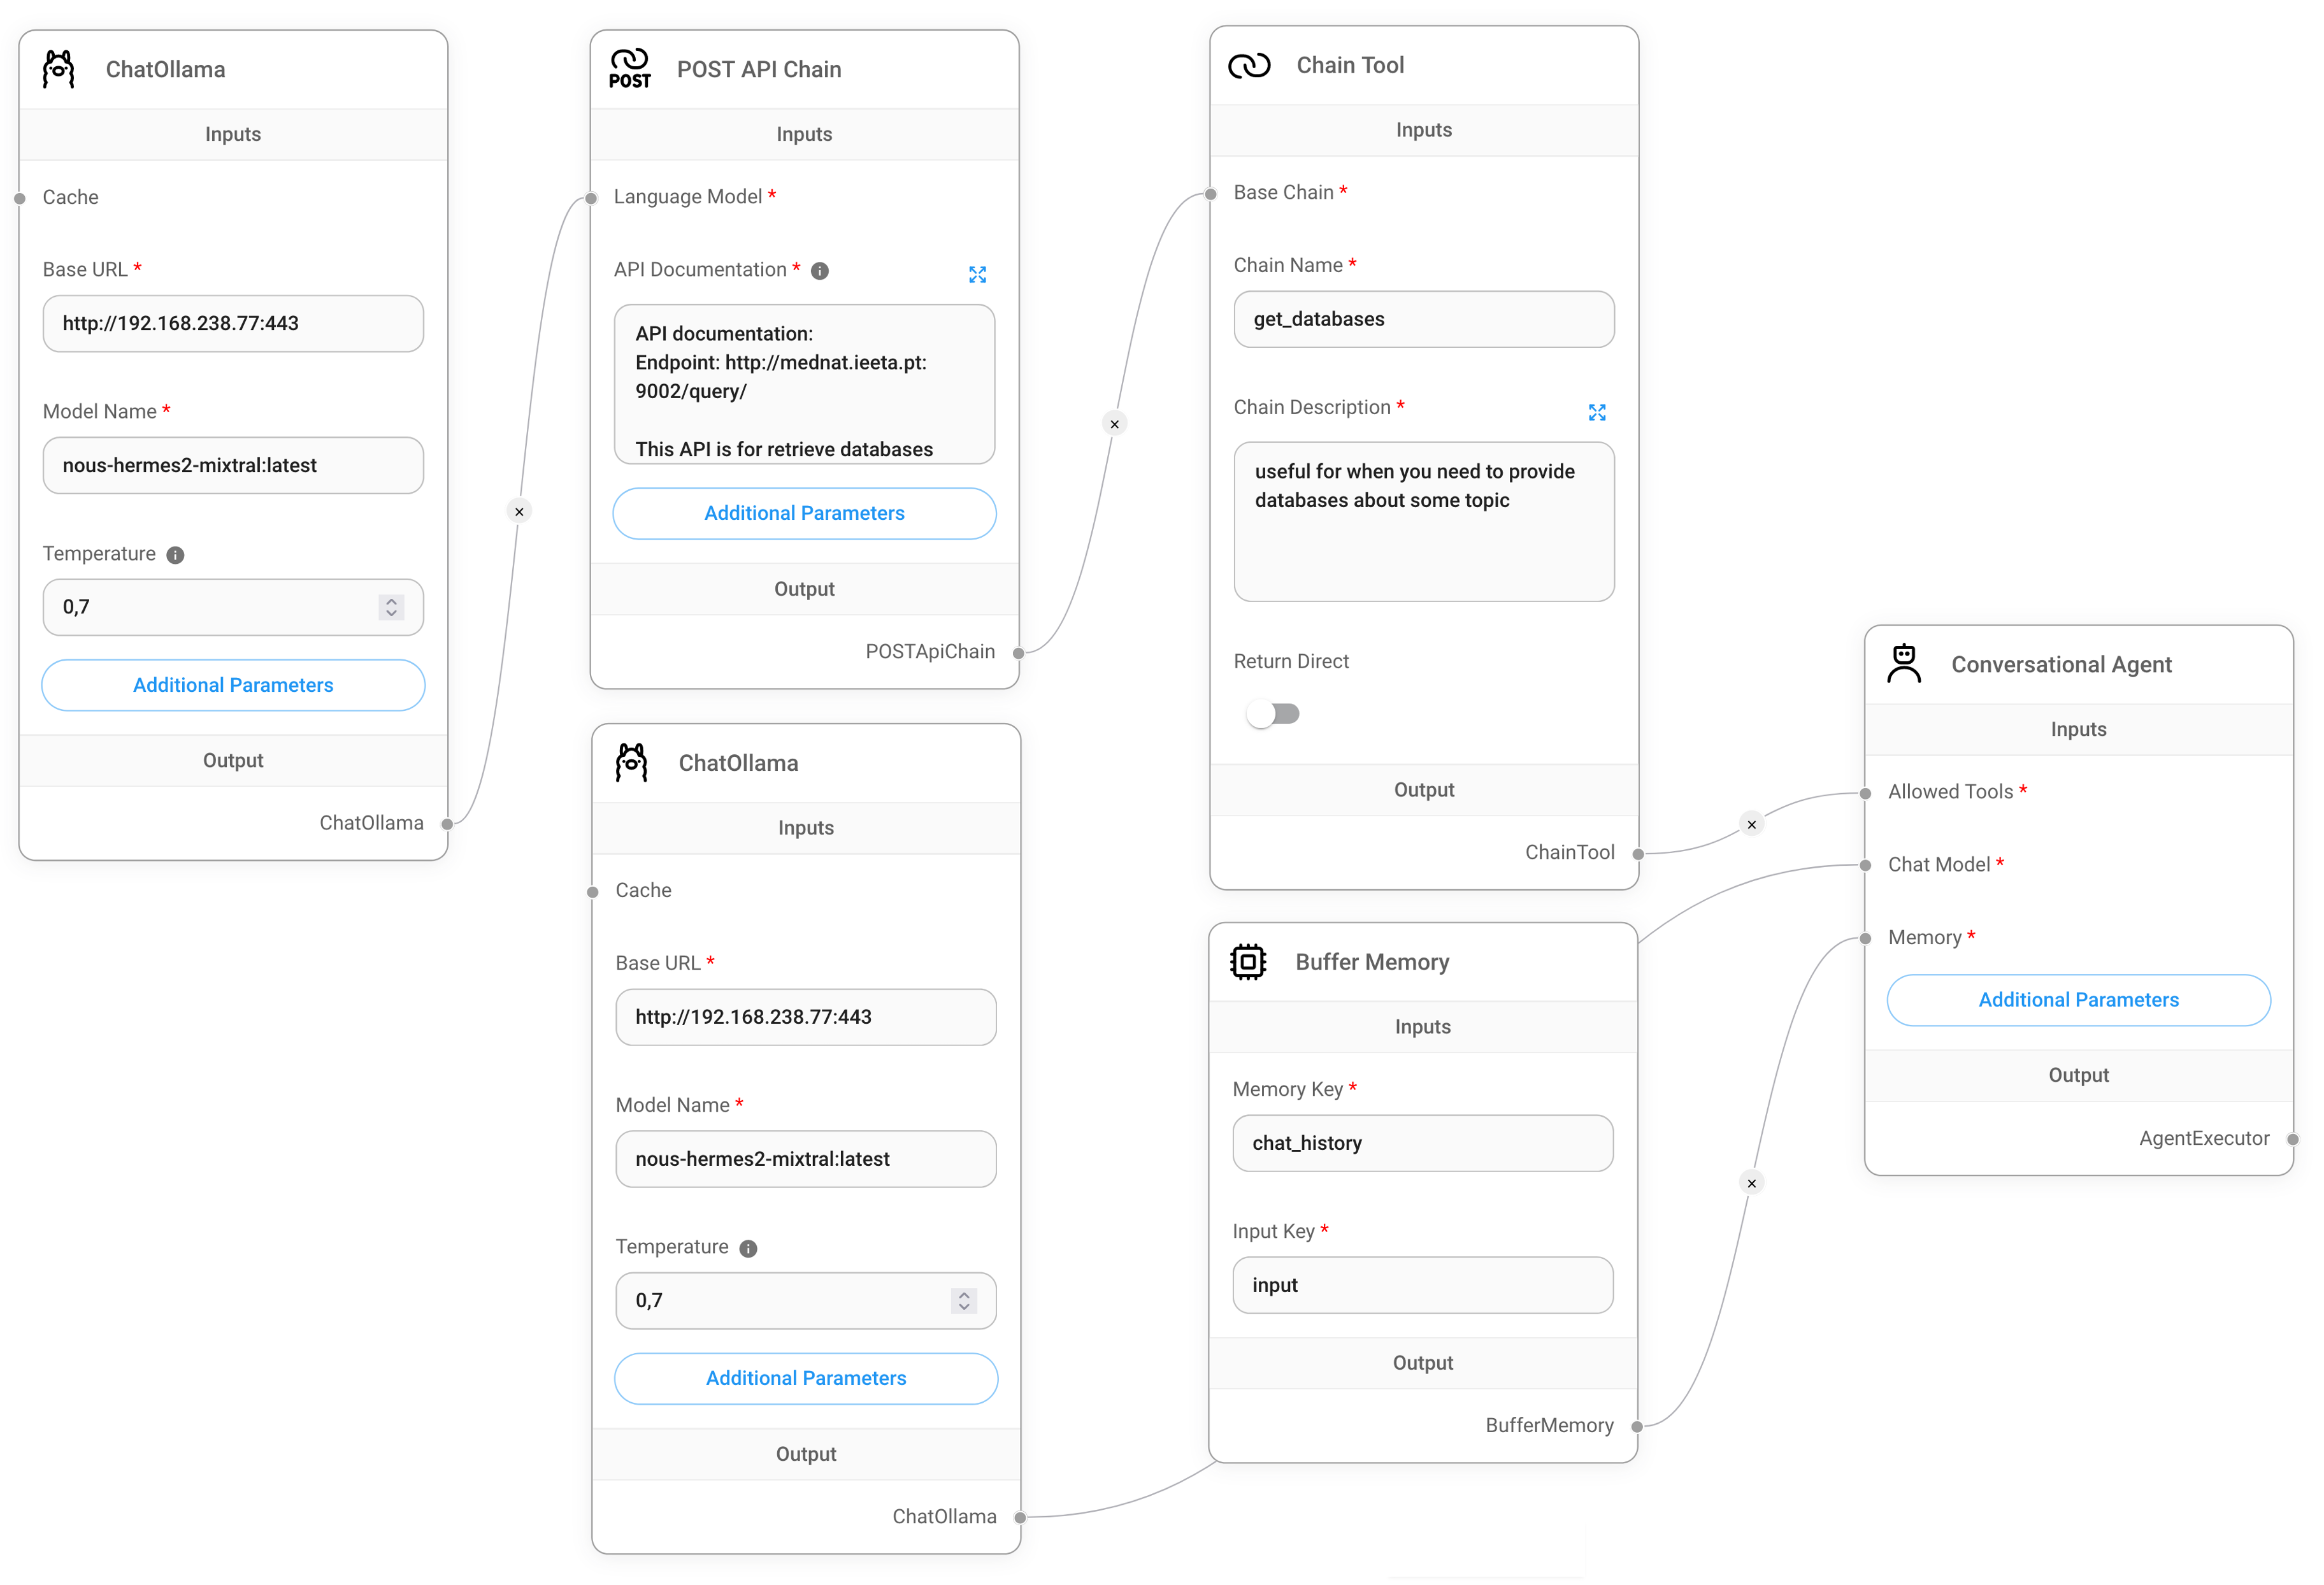
\includegraphics[width=\textwidth]{figs/chapter3/workflow.png}
    \centering
    \caption[Worflow implemented in FlowiseAI tool]{Worflow implemented in FlowiseAI tool.}
    \label{fig_workflow}
\end{figure}


The conversational agent employs a comprehensive approach to enable dynamic interactions on a healthcare {\ir} platform. It orchestrates the dialogue flow through the Conversational Agent Node, utilizing an {\llm} to provide a coherent and context-aware user experience. This node is configured with parameters that control tool access, chat model specifications, and memory capabilities, allowing it to maintain context or state information across interactions for structured conversations.

The core of conversational dynamics is powered by the ChatOllama Node, a chatbot engine designed for processing user queries and the generation of relevant responses. The implementation rely on Ollama since other solutions like ChatGPT API possess privacy issues. The Ollama operates based on a set of parameters including a base URL, alongside model specifications and a temperature setting that modulates probabilistic distribution over the predicted tokens. Furthermore, the Conversational Agent incorporates a Buffer Memory component, essential for the retention of interaction histories and stateful data. This component ensures the persistence of conversational context, a critical feature for enhancing user engagement and response relevance.

To provide the most relevant medical databases, a {\rag} architecture was adopted, as detailed in the section~\ref{rag_section}. This approach applied to this scenario involves retrieving the best databases from the {\ir} component and adding them to the {\llm} prompt. {\rag} enables the {\llm} to have up-to-date, valid, and domain-specific information to enhance response accuracy and relevance. 

The integration with the Chain Tool facilitates the application of prompt engineering techniques, enabling the agent to access the list of the recommended best databases. The tool consumes the endpoint of the {\ir} component, which is better described in the section~\ref{bm25implementation}. The conversational agent is equipped with real-time, accurate database recommendations, enhancing the quality of information provided to the user. 


\subsection{Langflow}

Langflow\footnote{\url{https://github.com/langflow-ai/langflow}} is another open-source tool to build {\ai} applications. It is also a low-code tool that allows the integration of {\llm} and {\ai} components. This tool simplifies the process of creating flows, such as chatflows. Users can drag components from the sidebar onto the canvas and connect them to begin building their applications. The platform allows for exploration by editing prompt parameters, grouping components into high-level components, and creating custom components. This intuitive interface makes Langflow a powerful tool for developing {\llm}-based applications.

% tbd: o que meto mais? não tenho implementação
An implementation was tested, but without much success due to some of the tool's limitations, such as the lack of basic functionalities like a conversational agent.

 


\oldsection[EHDEN chatbot architecture]{EHDEN chatbot architecture\protect\footnote{This section is mainly based in the publication \textit{A chatbot-like platform to enhance the
discovery of OMOP CDM databases, 34th Medical Informatics Europe Conference (MIE), 2024}}}


The system was designed to be integrated as a tool in the {\ehden} Portal. Therefore, authentication issues were solved by the current mechanisms available on this platform~\cite{almeida2024federated}. Therefore, the system was implemented to use the MONTRA2-SDK~\cite{almeida2024montra2}. This also provided the Network Dashboards tool, an interface to show the metadata, when researchers want to get more details about the suggested databases. 

The previous implementation, detailed in the section~\ref{flowise}, tried to adopt an open-source automation tool to build Chatbot applications, FlowiseAI~\cite{reis2024flowise}. However, these become limited to address the new requirements. Therefore, FlowiseAI was replaced by a Python-based backend, developed for this system. In addition to the {\ir} function, the backend also orchestrates chat flow between the various components. Figure~\ref{fig_arch} represents the key components of the system and their interconnections.

\begin{figure}[H]
    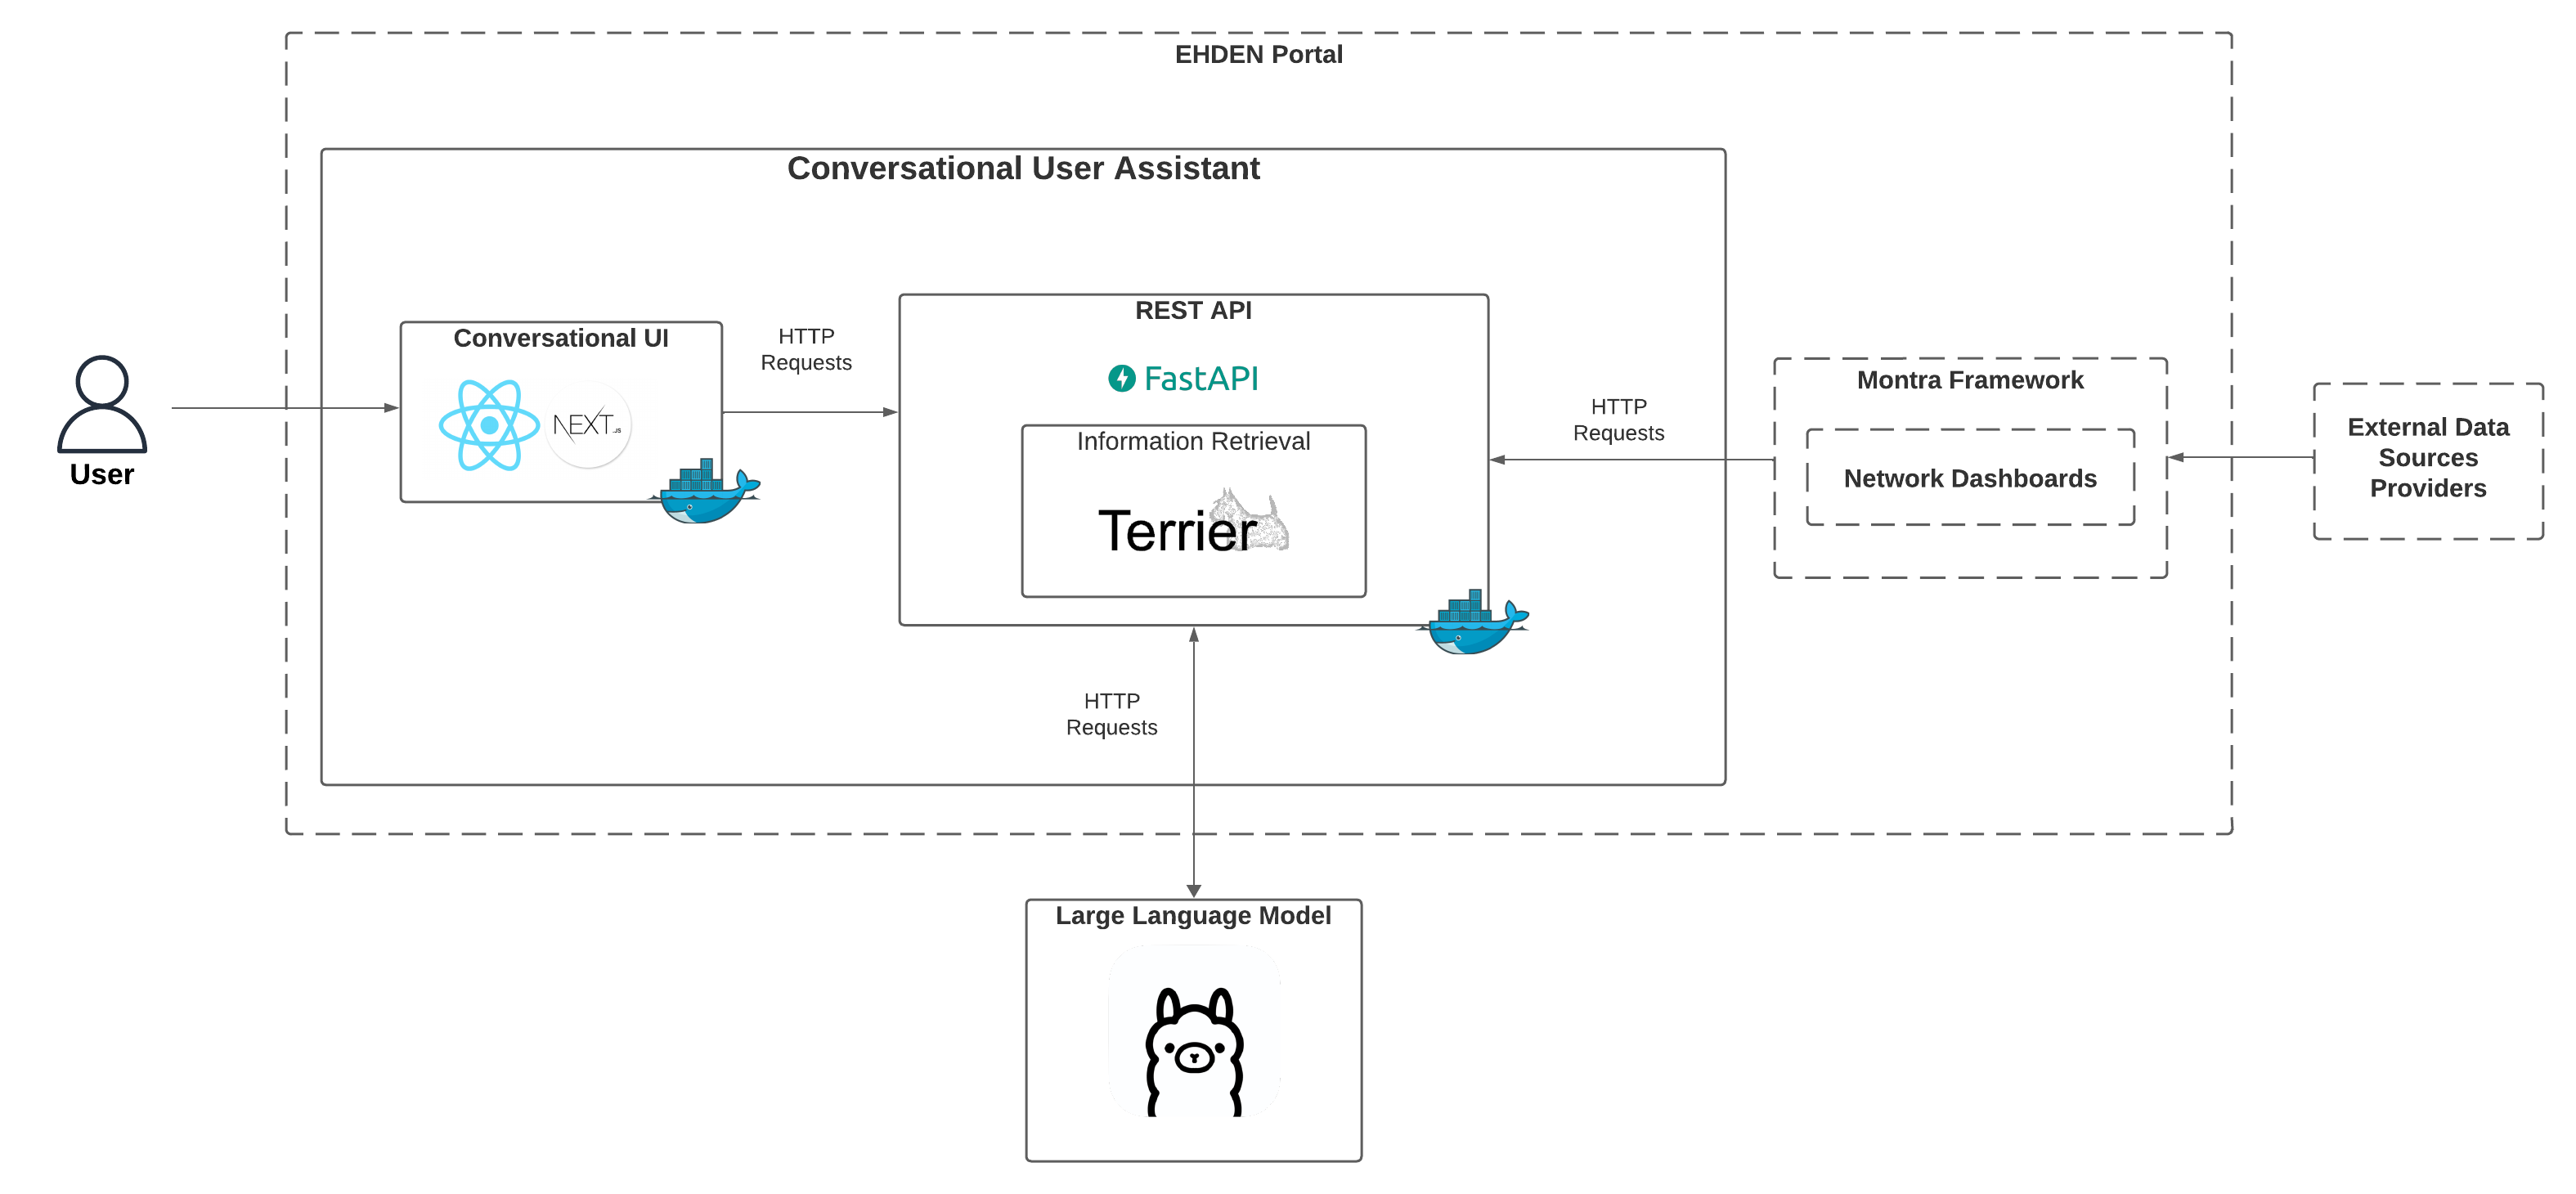
\includegraphics[width=1\textwidth]{figs/chapter3/architecture.png}
    \centering
    \caption[Overview of the chatbot architecture]{Overview of the EHDEN chatbot architecture.}
    \label{fig_arch}
\end{figure}

The Conversational User Interface is the primary interface for user interaction, built on the React framework. The User Interface records the user questions and conveys them to the backend to be processed in the component dedicated to {\ir}. 

The backend API, built on the FastAPI framework, handles the HTTP requests from the other components. When it receives a query from the User Interface, the backend communicates with the {\llm}. The {\llm} is the same open model detailed in the section~\ref{sec:llm}, \texttt{Nous Hermes 2 Mixtral 8x7B}. In this implementation, the {\llm} has two tasks: analyze the topic of health and generation of a response with databases or generate a simple response. If the first task returns false, \textit{i.e.}, if the user message is not related to health, the {\llm} generates a simple response reminding the user of the chatbot's purpose. Otherwise, if the first task is true, then the {\rag} architecture is applied. This means that the generation of a response with databases task is applied. The {\bm} retrieves the best databases to the {\llm}, so it could generate a response with that valid information.

For research purposes, researchers may save their conversations to facilitate data analysis and enhance their research outcomes. When a user decides to save a conversation, he can do so by pressing a save button, which triggers an API endpoint designed to store the conversation. The conversations are subsequently added to a JSON file, creating a structured and accessible format for future analysis. This method ensures that valuable data is systematically archived and easily retrievable for subsequent research endeavors.

Storing these dialogues can be particularly valuable for research purposes, for example, identify frequently asked questions by medical researchers. By analyzing the saved conversations, researchers can gain insights into common concerns, informational gaps, and the types of support often sought by medical researchers. By taking advantage of this stored information, the system can be improved, or even develop other platforms to improve the overall quality and impact of medical research.
